%!TeX root=./tese.tex
% Figures are generated by simulation/sweep_fig.py and simulation/
% burst_queue_fig.py into simulation/results/sweeps/ and copied into
% figuras/sim/ (prefixed sim_). Numbers come from progress/phase2-simulation.md
% (Results A-D) and simulation/results/sweeps/summary.json.
\chapter{The Two-Pool Simulation: Composition, Fidelity, and Saturation}
\label{cap:twopool}
\chaptermark{The Two-Pool Simulation}

The preceding chapters produced the three ingredients of the thesis's
experimental platform: a characterized workload
(Chapter~\ref{cap:trace-eda}), forecasts of its demand signals
(Chapter~\ref{cap:predictors}), and a silicon-calibrated cost model for the
vision stage (Chapter~\ref{cap:aiconfigurator}). This chapter composes them
into the running system the remaining experiments use: the full Azure trace
driving a vision pool costed on collected RTX~5090 silicon and a language
pool simulated by Dynamo's discrete-event engine under calibrated H100
timing. Three results are established. First, the language pool's timing
model matters: calibrated per-request timing exposes latency tails that the
simulator's default polynomial flattens. Second, the vision pool's cost
model admits an exact batching law --- encoder latency depends only on the
\emph{total} images per forward --- which grounds a realistic cross-request
batching policy and an analytic bound on the inter-pool handoff. Third, and
centrally: arrival-speedup sweeps locate each pool's saturation knee, and
the two knees sit far apart --- in \emph{opposite directions} on the steady
and bursty portions of the trace. The pools' decoupling, established
statistically in Chapter~\ref{cap:trace-eda}, is now a property of the
simulated serving system itself.

\section{Architecture: two pools, one seam}
\label{sec:sim-arch}

Dynamo's simulator (DynoSim/mocker) models text token processing only, so
the vision stage cannot live inside it. The composition instead runs the
vision pool as an event-driven FIFO of $C$ encoder workers \emph{inside the
workload converter}, costed per forward by AIC's encoder graph on the
collected \texttt{rtx\_5090} data, and hands the language pool to
\texttt{dynamo.replay}. The seam is the trace itself: an open-loop request
that spends $d$ milliseconds in the vision pool is equivalent to the same
request arriving at the language pool $d$ milliseconds later, so the
converter folds each request's encoder delay (queue wait + service +
handoff transfer) into its emitted arrival timestamp. A
\texttt{--no-encoder-shift} mode emits raw arrivals instead --- the
language pool in isolation --- which is what makes per-pool attribution
possible in the load sweeps below. The language pool runs offline with a
KV-aware router across two simulated workers; its per-request prefill and
decode times come either from the mocker's default polynomial or from AIC's
calibrated \texttt{h100\_sxm}/vLLM~0.22.0 database (the locked decoder-pool
platform), selected per run. Both pools therefore price work on the
platforms the thesis targets, and the entire pipeline is CPU-only and
deterministic given a trace window.

\section{Language-pool timing: the polynomial hides the tails}
\label{sec:sim-timing}

Table~\ref{tab:sim-poly-aic} compares the two timing models on the same
2{,}000-request steady window (raw arrivals, identical topology). The
calibrated model is moderately slower on averages and markedly heavier in
the tails: TTFT p99 grows $1.24\times$ and the maximum TTFT and inter-token
latency roughly double ($1.8\times$ and $1.9\times$). Burst behavior ---
precisely what autoscaling experiments measure --- is visible only under
calibrated timing, so all headline runs use AIC timing and the polynomial
is retained for cheap coverage sweeps. One measurement note: these AIC
numbers come from the source-built runtime, whose calibrated predictions
run in-core (Rust) in microseconds; an earlier wheel-based runtime ran them
as per-request Python callbacks whose wall-time leaked into the simulated
clock, inflating the \emph{extreme} tail only (identical p99, maximum TTFT
7.6 vs.\ 4.5~s on identical perf data) --- an instrumentation artifact to
guard against when a simulator's timing hook is slower than the events it
prices.

\paragraph{Family transfer.} The language-pool numbers in this chapter are
for Qwen3-VL-8B at TP1. A spot-check prices the family flagship,
Qwen3-VL-235B-A22B at TP8 (MoE-TP~8), on the same shipped H100 data, window,
and topology: TTFT p99 of 398 / 1{,}402~ms at $1\times$/$4\times$ the trace
rate against the 8B's 307 / 882, with $2\times$ the decode latency
throughout (TPOT 14.9 vs.\ 7.9~ms; 87 vs.\ 142 output tok/s per user).
Under the evaluation SLA the decode bound is what moves: the flagship's ITL
p99 is already \SI{87.7}{\milli\second} at the trace's own rate, so its
knee sits at $s{=}1$ ($2.8$~req/s) against the 8B's $s{=}2$ --- decoder
scale halves the language pool's operating envelope while leaving the
vision pool untouched. The vision
side needs no such caveat: the ViT \emph{and} its 4096-dimensional projector
output are identical between the 8B and the 235B
(Chapter~\ref{cap:aiconfigurator}), so the encoder cost model, the batching
law, the burst-saturation result, and the handoff bound all transfer to the
flagship unchanged.

\begin{table}[htb]
\centering
\caption{Language pool under identical load and topology, polynomial vs.\
calibrated (AIC \texttt{h100\_sxm}, vLLM 0.22.0) timing; 2{,}000-request
steady window, 2 workers, offline KV router.}
\label{tab:sim-poly-aic}
\small
\begin{tabular}{lrr}
\toprule
Metric & Polynomial & AIC h100 \\
\midrule
TTFT avg / p99 / max (ms) & 67.3 / 248 / 2{,}540 & 68.2 / 307 / 4{,}518 \\
Request latency avg / p99 (ms) & 1{,}413 / 6{,}879 & 1{,}590 / 8{,}163 \\
Inter-token latency avg / max (ms) & 6.79 / 181 & 7.67 / 348 \\
Output tok/s per user (avg) & 160.6 & 142.0 \\
\bottomrule
\end{tabular}
\end{table}

{\renewcommand{\sectionmark}[1]{}%
\section{Encoder-pool realism: an exact batching law and a handoff bound}%
\label{sec:sim-encoder}}
\sectionmark{Encoder-pool realism}

Two fidelity upgrades make the vision pool defensible rather than merely
plumbed.

\paragraph{Batching.} Probing AIC's encoder graph shows its predicted
latency is \emph{exactly} a function of the total images in a forward:
every factoring of $N$ images into (batch, images-per-request) --- $(1,64)$,
$(2,32)$, $(64,1)$ --- returns the same latency to the microsecond, because
attention is evaluated at the product batch$\times$images and every other
operator at the total token count. Batching is therefore modeled by costing
each dispatched batch at its image total, and it pays: $f(1) = \SI{8.16}{\milli\second}$
per image alone versus $f(64) = \SI{316.4}{\milli\second}$ ---
\SI{4.94}{\milli\second} per image amortized, a $1.65\times$ throughput gain
that amounts to a ${\sim}\SI{3.2}{\milli\second}$ fixed per-forward
overhead. (Measured end-to-end, the realized gain is smaller and
saturates by $N{\approx}6$--$8$ --- the model-versus-silicon band of
Section~\ref{sec:aic-model-vs-silicon}, conservative for the saturation
results below.) The pool's dispatch policy is greedy FIFO: a freed worker takes
whole queued requests, in order, up to a 64-image cap (the collected batch
range, so no extrapolation); a request exceeding the cap alone --- the
trace reaches $97^2 = \num{9409}$ images --- is chunked into $\leq
64$-image forwards that enter the FIFO as independent dispatch units, so
several free workers drain one oversized request concurrently. This
chunk-parallel policy is physically grounded --- images are independent in
the encoder, and the batching law prices any forward at its image total
--- and it is what makes encoder tail latency \emph{capacity-controllable}:
under the sequential alternative (one request's chunks chained on one
worker, retained behind a converter flag), the largest requests carry an
intrinsic multi-second service floor that no worker count removes ---
measured on the fastest-onset episode, delay p99 plateaus at
\SI{2.9}{\second} from 4 through 32 workers --- which would make every
frames-heavy window statically infeasible under the evaluation SLA by
construction. The largest request still costs ${\approx}\SI{46}{\second}$
of kernel time (147 forwards), but spread across whatever workers are
free. Under low load a lone request dispatches immediately, reproducing
per-request behavior; the policy changes nothing at the steady head
(delay percentiles identical to three decimals) and matters exactly where
batching should --- inside bursts.

\paragraph{Handoff.} The encoder's output must cross pools: post-merge
vision embeddings of $196 \times 4096$ bf16 values per image ---
${\approx}\SI{1.6}{\mega\byte}$ per image, \SI{194}{\mega\byte} for a
121-image request. The simulation bounds this analytically as
$\text{RTT} + \text{bytes}/\text{bandwidth}$ on a parameterized link
(default \SI{25}{Gbps}): \SI{0.71}{\milli\second} at the median request of
the steady window, \SI{62}{\milli\second} at its 121-image maximum. The
transfer is charged to request latency but not to the worker (asynchronous
DMA/NIC) --- optimistic for encoder throughput, conservative for latency.
A measured NIXL transfer curve can later replace the bound without
touching anything downstream. The trace records no image sizes, so the
uniform 448\textsuperscript{2} assumption of
Chapter~\ref{cap:aiconfigurator} stands, with its known, bounded
${\sim}1.14\times$ conservative bias on comparable ViT work.

{\renewcommand{\sectionmark}[1]{}%
\section{Saturation knees: the decoupling, now in simulation}%
\label{sec:sim-knees}}
\sectionmark{Saturation knees}

With both pools defensibly timed, the load question becomes answerable:
\emph{at what offered load does each pool violate its latency target?}
Arrival timestamps are compressed by a speedup factor $s$ --- natively in
\texttt{dynamo.replay} for the language pool (on the isolation trace, so
the knee is attributable to that pool alone), in the converter for the
vision pool --- and each pool is graded against the thesis's evaluation
SLA, deliberately tail-based because burst-time tails are precisely the
failure mode under study: the language pool must hold TTFT p99
$<\SI{1}{\second}$ \emph{and} inter-token latency p99 $<\SI{100}{\milli\second}$
(first token within a second and at least 10~tokens/s for the worst
percentile user); the vision pool must hold encoder delay p99
$<\SI{1}{\second}$, matching the language TTFT budget so a composed
multimodal request stays within ${\approx}\SI{2}{\second}$ p99 to first
token. (The reactive baseline of the next chapter regulates on Dynamo's
native \emph{window-mean} targets, $500/\SI{50}{\milli\second}$ --- that is
its control law, evaluated like every other policy against the bounds
above.) Two windows are swept at the locked 2-encoder $\times$ 2-LLM
topology: the steady 2{,}000-request head (\SI{2.77}{req/s},
\SI{8.0}{img/s}) and the week's largest burst episode
(Section~\ref{sec:eda-vision}: 64{,}804 requests over \SI{8.3}{\hour},
mean \SI{2.17}{req/s} but \SI{116}{img/s}, peaking at \SI{370}{img/s}).
Figure~\ref{fig:sim-knees} shows every curve; Table~\ref{tab:sim-knees}
the knees.

\begin{table}[htb]
\centering
\caption{Saturation knees per pool and window under the evaluation SLA:
the largest swept speedup $s$ meeting every bound, and that knee's offered
load. ``ITL-bound'' marks knees whose successor point still meets the TTFT
budget but crosses the inter-token bound --- decode saturates the SLA
before prefill queueing does. The vision pool's steady-window knee is
censored (never crossed within the swept range); on the burst window it is
saturated at the trace's own recorded rate.}
\label{tab:sim-knees}
\footnotesize
\setlength{\tabcolsep}{3pt}
\begin{tabular}{llrrr}
\toprule
Pool / timing & Window & Knee & Offered & TTFT p99 (ms), $1{\to}$knee \\
\midrule
LLM / poly & steady & $s{=}2$ (ITL-bound) & 5.5 req/s & $249 \to 277$ \\
LLM / AIC  & steady & $s{=}2$ (ITL-bound) & 5.5 req/s & $307 \to 418$ \\
LLM / poly & burst & $s{=}1$ & 2.2 req/s & $910$ at $s{=}1$ \\
Vision / AIC & steady & $\geq s{=}32$ (cens.) & $\geq$ 256 img/s & $199 \to 787$ \\
Vision / AIC & burst & \textbf{none: over at $s{=}1$} & 116 img/s & $5{,}013$ at $s{=}1$ \\
\bottomrule
\end{tabular}
\end{table}

\begin{figure}[htb]
\centering
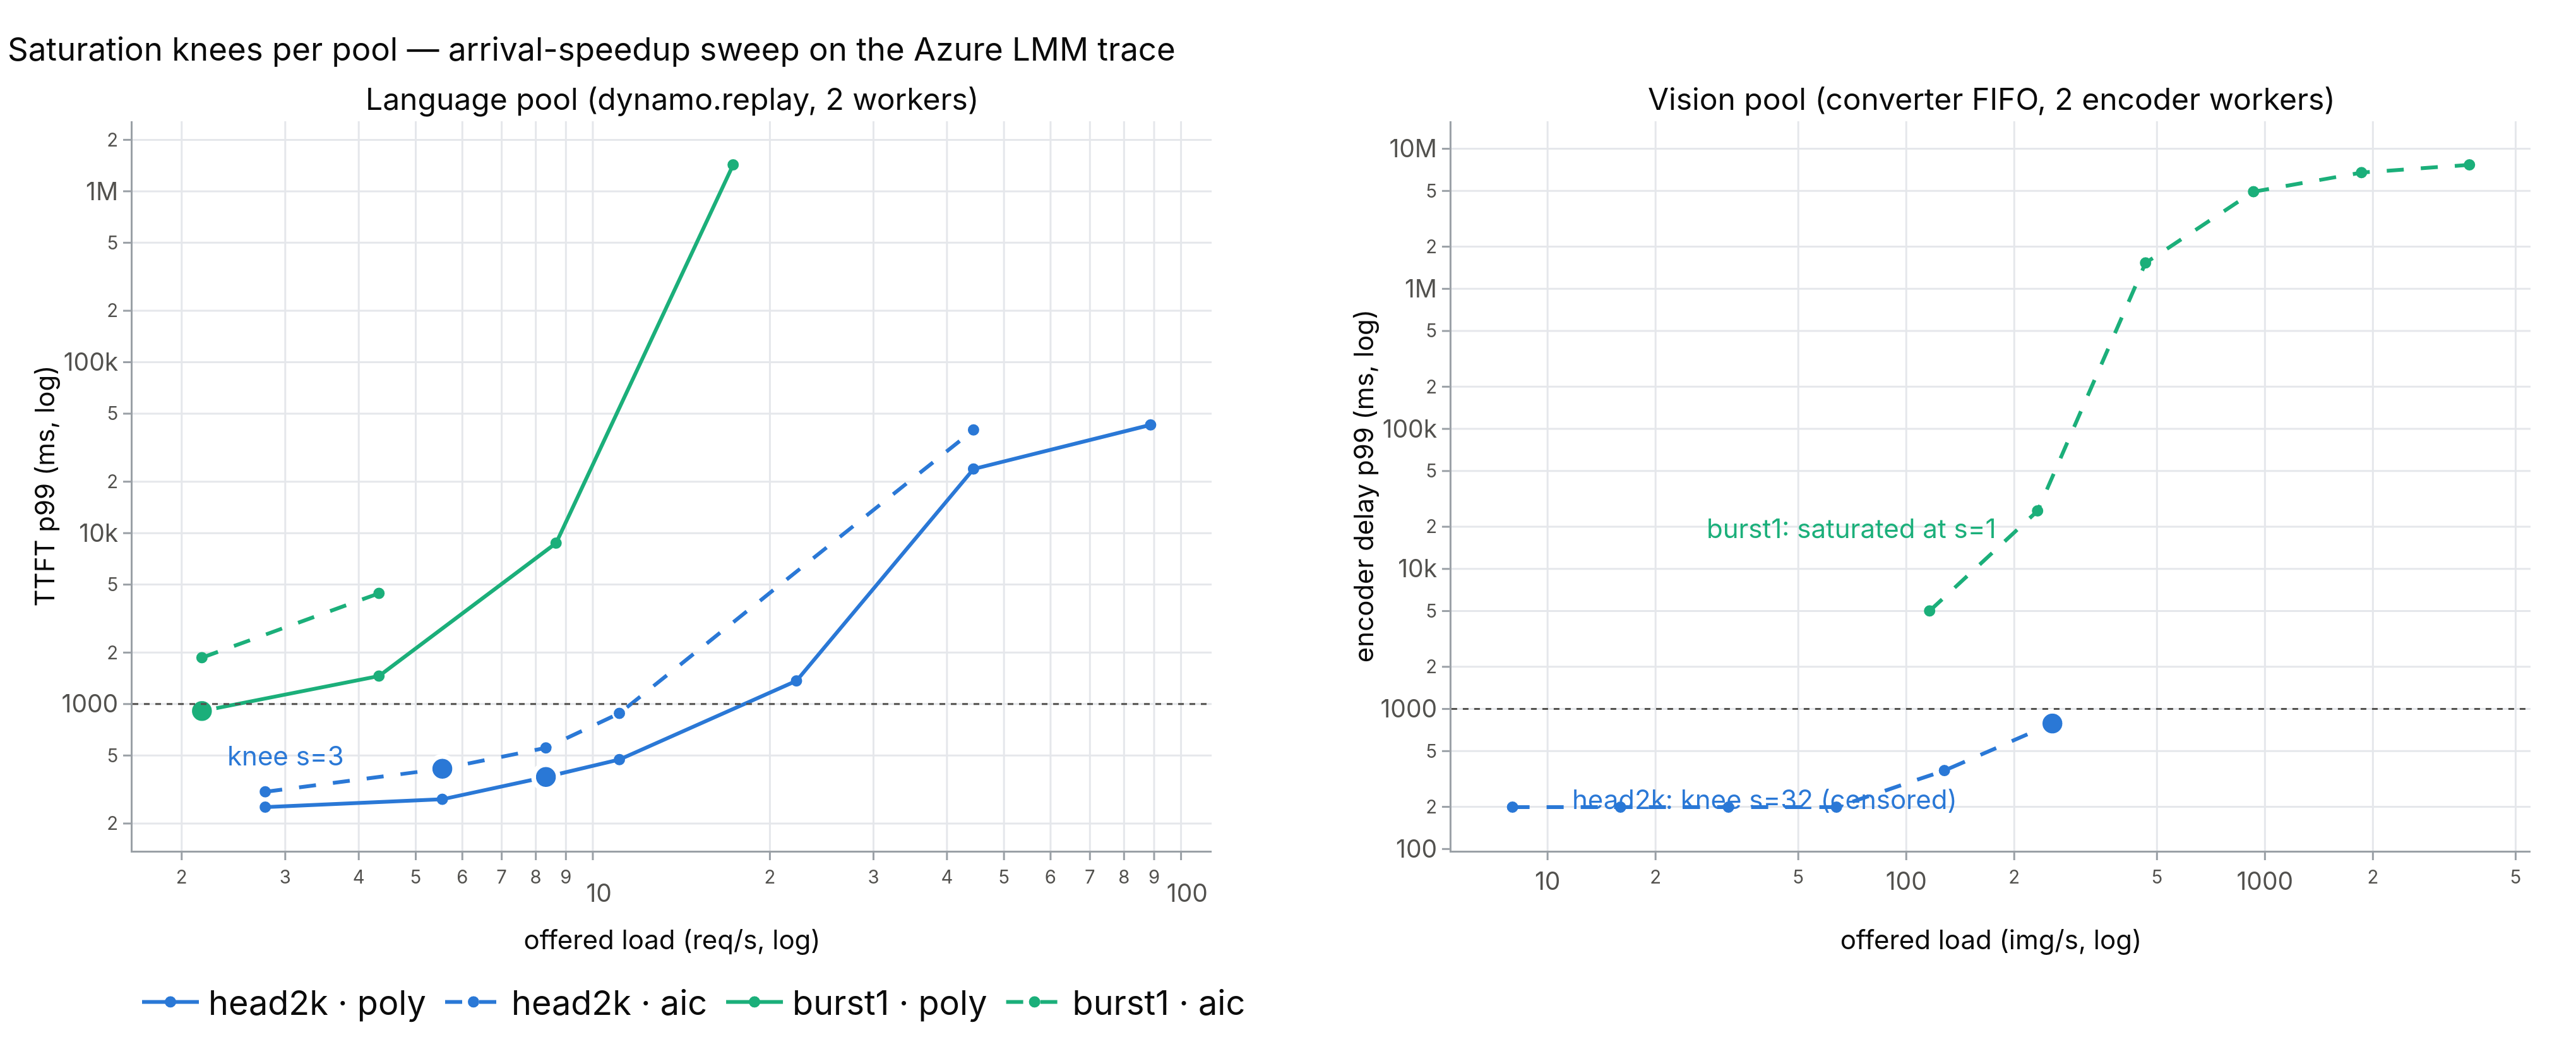
\includegraphics[width=\linewidth]{figuras/sim/sim_knees.png}
\caption{TTFT and encoder-delay p99 versus offered load per pool
(log--log), swept by arrival speedup at the fixed 2$\times$2-worker
topology; knee markers apply the full evaluation SLA, so the language
knees sit \emph{below} the TTFT line --- they are set by the inter-token
bound (``ITL-bound''), which crosses first. On the steady window (blue)
both timing models put the language knee at $s{=}2$ while the vision pool
remains under its bound through $s{=}32$ --- at the language pool's knee
the encoder idles at 4.5\% utilization. On the burst episode (green) the
order reverses: the vision pool starts \emph{above} its bound at the
episode's own recorded rate, which the language pool still meets. No
single load axis serves both pools.}
\label{fig:sim-knees}
\end{figure}

The two knees differ on both windows, in opposite directions. On the
steady head the vision pool carries at least $16\times$ the language
pool's load headroom (both timing models) --- sizing both pools off one
signal would overprovision the encoder fleet by an order of magnitude in
calm traffic. A second structural fact falls out of the dual-bound SLA:
the language pool is \emph{decode-bound}, not TTFT-bound --- at the knee's
successor point the TTFT budget still has $2\times$ slack while ITL p99
has crossed ($154$ and \SI{211}{\milli\second} for polynomial and
calibrated timing at $s{=}4$) --- so language-pool capacity under an
interactive SLA is set by sustained token throughput per user, exactly the
axis the 235B spot-check of Section~\ref{sec:sim-timing} stresses further.
On the burst episode the asymmetry flips: the vision pool violates its
bound \emph{at the trace's own recorded rate}, with a p99 encoder delay of
\SI{5.0}{\second} --- while its mean utilization is only 29\%, and while
the language pool, fed the very same requests, still meets the full SLA at
that rate (its knee: $s{=}1$; at $2\times$ both bounds fail).

Figure~\ref{fig:sim-burst-queue} exposes the mechanism. The episode's
7{,}716 frames-class requests (${>}64$ images each) decompose into
83{,}432 chunk forwards --- every forward at most \SI{315}{\milli\second}
--- and arrivals clump: the worst second lands 975 images at once. Behind
a strict FIFO, a frames flood therefore monopolizes \emph{every} worker at
once: the backlog exceeds 1{,}000 queued images for 805 seconds spread
across the eight-hour episode, peaking at 4{,}701, each excursion a
multi-second p99 event, yet the pool drains fully between excursions and
ends the window with an empty queue. This is the provisioning
gap in its sharpest form: a monitor watching request rate
(\SI{2.2}{req/s}, unremarkable), mean utilization (29\%), or any
minute-averaged signal sees a healthy pool, while the tail SLA is being
violated episodically all day. Catching it requires watching --- or
forecasting --- the image signal itself, at exactly the horizons
Chapter~\ref{cap:predictors} showed to be forecastable.

\begin{figure}[htb]
\centering
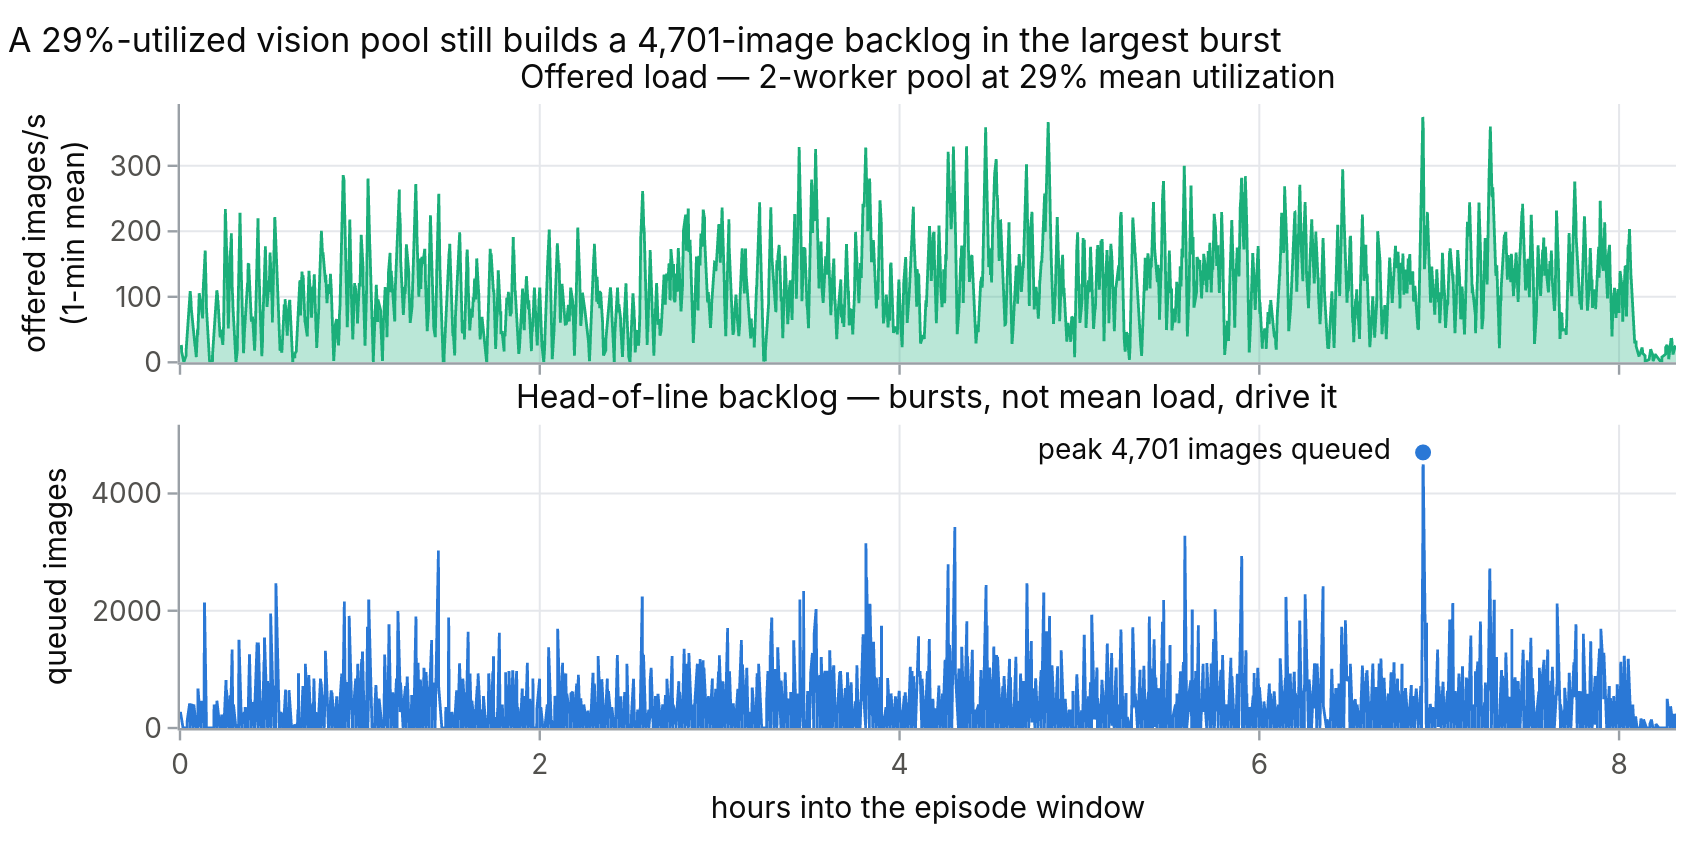
\includegraphics[width=\linewidth]{figuras/sim/sim_burst_queue.png}
\caption{Inside the burst episode at the trace's own rate: offered image
load (top, 1-minute mean of the per-second series) and the encoder pool's
queued-image depth (bottom, per second). The queue repeatedly spikes past
1{,}000 images --- peaking at 4{,}701 --- and fully drains between spikes,
so the episode's \emph{mean} utilization stays at 29\% while p99 encoder
delay reaches \SI{5.0}{\second}: episodic FIFO head-of-line blocking by
frames-class floods, invisible to rate- or mean-utilization monitoring.}
\label{fig:sim-burst-queue}
\end{figure}

\section{Limitations}
\label{sec:sim-limitations}

The evaluation SLA's specific bounds (\SI{1}{\second}/\SI{100}{\milli\second}/%
\SI{1}{\second}) are a design choice --- defensible for interactive
multimodal serving, but the knee positions shift with them (under a lax
TTFT-only \SI{2}{\second} bound the language knees sit one to two octaves
higher); the sweep curves themselves are SLA-free and re-derivable under
any bounds. The topology is locked at 2$\times$2 workers here --- the
worker-count grid is the static-optimal baseline's search space, not this
chapter's --- and language-pool results are reported for the 8B at TP1 with
a 235B-TP8 spot-check (Section~\ref{sec:sim-timing}); intermediate family
members (32B) were not priced. The vision pool inherits the uniform-448\textsuperscript{2}
image assumption and AIC's ${\sim}1.14\times$ conservative encoder bias;
the handoff term is an analytic bound, not a measured NIXL curve. Encoder
delays fold into language-pool arrivals through the trace seam, which
serializes the pools per request (no speculative overlap of encoder and
prefill work). Finally, per-pool knees were measured with the other pool
absent by construction (isolation trace / converter-only), which is what
makes them attributable --- composed-system interaction effects at high
load remain for the baseline runs.

\section{Summary}

The two-pool simulation now runs the real trace end to end on calibrated
timing for both pools: an encoder pool whose batching follows an exact,
probe-verified cost law with a bounded inter-pool handoff, and a language
pool whose calibrated timing surfaces the latency tails the default
polynomial hides. Stressed with arrival-speedup sweeps under a tail-based interactive SLA,
the composed system reproduces the thesis's motivating claim as measured
behavior: the pools saturate at loads $\geq 16\times$ apart on steady
traffic --- with the language pool decode-bound, not TTFT-bound --- and in
the \emph{opposite} order during the largest burst, where the vision pool
violates its tail bound at the trace's own rate and 29\% mean utilization
while the language pool still meets the full SLA. A single scaling signal
cannot serve both pools, and the signal that matters for the vision pool
is invisible to rate- and utilization-based monitors. The next chapters
build the baselines (static-optimal sizing and the reactive planner) on
this platform and then close the loop with the per-pool forecasts of
Chapter~\ref{cap:predictors}.
